\documentclass
    [ ngerman
    , BCOR=10mm
    , openright
    , parskip=half
    , 11pt
    , oneside
    % , draft
    ]{scrreprt}

\usepackage{scrhack}
\usepackage{lmodern}
\usepackage[utf8]{inputenc}
\usepackage[T1]{fontenc}
\usepackage{datetime}
\usepackage[backend=biber,style=authoryear]{biblatex} % style=alphabetic
\usepackage[a4paper,top=3cm, bottom=3cm]{geometry}
\usepackage{setspace}
\usepackage[automark]{scrpage2}
\usepackage[multiple]{footmisc}
\setcounter{secnumdepth}{3}
\setcounter{tocdepth}{3}
% \usepackage{fancyhdr}
\usepackage{lipsum}
\usepackage{microtype}
\usepackage[clearempty]{titlesec}
\usepackage[ngerman]{babel}
\usepackage{acronym}
\usepackage{array}
\usepackage{pst-pdf}
\usepackage{multicol}
\usepackage[german]{algorithm2e}
\usepackage{yhmath}
\usepackage{amsmath}
\usepackage{subfig}
\usepackage{wrapfig}
\usepackage{blindtext}
\usepackage[colorlinks=false, pdfborder={0 0 0}]{hyperref}

\usepackage{graphicx}
\graphicspath{{./img/}}

\usepackage[german,vario]{fancyref}

%%%%%%%%%%%%%%%%%%%%%%%%%%%%%% User specified LaTeX commands.
%% http://www.schlosser.info/in-latex-mit-varioreffancyref-automatisch-ab-seite-statt-auf-seite-setzen/
\makeatletter
\let\@f@ref@sav=\@f@ref
\renewcommand*{\@f@ref}[4]{%
  \def\@curtlabtype{#3}%
  \protect\@f@ref@sav{#1}{#2}{#3}{#4}%
}%
\addto\extrasngerman{%
  \renewcommand\reftextfaraway[1]{%
    \ifthenelse{\equal{\@curtlabtype}{chap}}{ab Seite}{auf Seite}~\pageref{#1}}%
  \renewcommand\reftextafter{%
    \ifthenelse{\equal{\@curtlabtype}{chap}}{ab der nächsten Seite}{auf der nächsten Seite}}%
}
\makeatother
%% src: http://tex.stackexchange.com/a/70847
\newcommand*{\fancyreflstlabelprefix}{lst}

\fancyrefaddcaptions{german}{%
  \providecommand*{\freflstname}{Quelltext}%
  \providecommand*{\Freflstname}{Quelltext}%
}

\frefformat{plain}{\fancyreflstlabelprefix}{\freflstname\fancyrefdefaultspacing#1}
\Frefformat{plain}{\fancyreflstlabelprefix}{\Freflstname\fancyrefdefaultspacing#1}

\frefformat{vario}{\fancyreflstlabelprefix}{%
  \freflstname\fancyrefdefaultspacing#1#3%
}
\Frefformat{vario}{\fancyreflstlabelprefix}{%
  \Freflstname\fancyrefdefaultspacing#1#3%
}

%%%% format
\setlength{\parindent}{3em}
\setlength{\parskip}{\baselineskip}
% \onehalfspacing
% Layout
\pagestyle{scrheadings}
%\pagestyle{empty}
\clubpenalty = 10000
\widowpenalty = 10000
\displaywidowpenalty = 10000
\hbadness = 10000

%% Definitions
\newcommand{\projname}{VM-SVOGI}
\newcommand{\titel}{Virtual Mapping for Sparse Voxel Global Illumination}
\newcommand{\untertitel}{Virtual Mapping for Sparse Voxel Global Illumination}
\newcommand{\authorname}{Jan-Philip Loos}
\newcommand{\thesisname}{Master Thesis}
\newcommand{\institute}{Fachhochschule Wedel}
\newcommand{\Datum}{XXXX xx, 2015}
\newcommand{\chpref}[1]{chapter~\ref{#1}}


\ifpdf
  \usepackage{hyperref}
  \definecolor{darkblue}{rgb}{0,0,.5}
  \hypersetup
    { colorlinks=true
    , breaklinks=true
    , linkcolor=darkblue
    , menucolor=darkblue
    , urlcolor=darkblue
    , pdftitle={\projname -- \untertitel}
    , pdfsubject={\thesisname}
    , pdfauthor={\authorname}
    }
  \usepackage{pdflscape}
\else
  \usepackage{lscape}
\fi

%% Listings %%%%%%%%%%%%%%%%%%%%%%%%%%%%%%%%%%%%%%%%%%%%%%%%%%%%%%%%%
\usepackage{listings}
\usepackage{sourcecodepro} % now the default typewriter font
\KOMAoptions{listof=totoc} % necessary because of scrhack
\renewcommand{\lstlistlistingname}{Quelltextverzeichnis}
\renewcommand{\lstlistingname}{Quelltext}
\lstset
  { basicstyle=\tiny\ttfamily\footnotesize
  , breaklines=true
  , captionpos=b
  , showstringspaces=false
  , keywordstyle=\color{blue}
  , backgroundcolor=\color{black!3}
  }

% \lstnewenvironment{inlinehaskell}
% {\spacing{1}\lstset{language=haskell,nolol,aboveskip=\bigskipamount}}
% {\endspacing}

\lstnewenvironment{haskell}[1][]{
    \noindent
    \minipage{\linewidth}
    \vspace{0.5\baselineskip}
    \lstset
        { basicstyle=\footnotesize\ttfamily
        , language=Haskell
        , tabsize=2
        , frame=single
        , #1
        }
}{\endminipage}

\newcommand{\haskellinput}[2][]{
  \begin{spacing}{1}
  \lstinputlisting[language=Haskell,nolol,aboveskip=\bigskipamount,#1]{#2}
  \end{spacing}
}

\lstMakeShortInline[columns=fixed,language=Haskell]|
% \newcommand{\inlinehaskell}{
%   \lstinline[language=Haskell]
% }

\newcommand{\haskellcode}[2][]{\mylisting[#1,language=Haskell]{#2}}

\newcommand{\mylisting}[2][]{
\begin{spacing}{1}
\lstinputlisting[basicstyle=\footnotesize\ttfamily, frame=lines,tabsize=2,aboveskip=2\bigskipamount,#1]{#2}
\end{spacing}
}


\addbibresource{bib/haskell-engine.bib} 

\begin{document}
\pagenumbering{roman}

% \pagestyle{plain}
\pagestyle{scrheadings}
% \pagestyle{fancy}


%%%%%%%%%%%%%%%%%%%%%%%%%%%%%% Titlepage
\titlehead{
  \centering
  
\includegraphics[width=.5\textwidth]{img/fhw}\\
  \bigskip
  \textsc{\Large Fachbereich Informatik}
}

\subject{\thesisname}
\title{\titel}
\subtitle{\Large \untertitel}
\date{\vspace{-1cm}{\small Eingereicht:}\\\medskip\Datum}
\author{}
\publishers{\vfill
  \normalsize
  \begin{minipage}{13cm}
  
    \raggedright
    {\small Eingereicht von:} \\
    \smallskip
    {\Large \authorname\ (Mat.-Nr.: 9912)}\\
     Kielmannseggstra{\ss}e 65\\
     22043 Hamburg\\
     Tel.: (+49)~160~966\,511\,88\\
     E-mail: jloos@maxdaten.io\\
     \medskip
     Fachsemester: \warn{XX}\\
     Semester: \warn{XX}\\

    
    \bigskip
    \bigskip
       
    \begin{multicols}{2}
      \raggedright
      {\small Referent:}\\
      \smallskip
      {\Large Prof. Dr. C.-A. Bohn}\\
      Fachhochschule Wedel\\
      Feldstraße 143\\
      22880 Wedel\\
      Phone: 00000000\\
      E-mail: bo@fh-wedel.de\\
         
      \raggedleft
      {\small Korreferent:}\\
      \smallskip
      {\Large Prof. Dr. Uwe Schmidt}\\
      Fachhochschule Wedel\\
      Feldstraße 143\\
      22880 Wedel\\
      Phone: (041\,03)~80\,48-45\\
      E-mail: si@fh-wedel.de\\
    \end{multicols}
 \end{minipage}
}

\maketitle

% our back titlepage
\begin{titlepage}
\centering
{\huge \titel}\bigskip\\  
{\Large \untertitel}\bigskip\\
{\large \thesisname\ von\ \authorname}\bigskip\\
\KOMAoptions{titlepage=false}
\begin{abstract}
\warn{\blindtext}
\end{abstract}
\par\vfill
\authorname \bigskip\\
\ccbysa\\
Dieses Werk ist lizenziert unter einer Creative Commons Namensnennung\\
Weitergabe unter gleichen Bedingungen 4.0 International Lizenz.\bigskip\\
Layout done with {\rmfamily \LaTeXe}, {\sffamily \KOMAScript} and {\rmfamily B\textsc{ib}\LaTeX}.
\end{titlepage}
\clearpage

% \cleardoublepage

%%% blank site
\thispagestyle{empty}
\null\newpage


%%%%%%%%%%%%%%%%%%%%%%%%%%%%%% Table of Content

\thispagestyle{empty}
\tableofcontents
% \cleardoublepage

%%% blank site
\thispagestyle{empty}
\null\newpage


\listoffigures
\listoftables
\lstlistoflistings
\chapter{Abkürzungsverzeichnis}
\begin{acronym}
    \acro{PBR}{Physically Based Rendering oder Physically Based Shading}
\end{acronym}
% \cleardoublepage

\thispagestyle{headings}
\pagenumbering{arabic}


%%%%%%%%%%%%%%%%%%%%%%%%%%%%%% Einführung
\chapter{Einführung und Wegweiser}

Diese Einführung dient als Wegweiser durch diese Arbeit und soll einen kurzen Überblick über die folgenden Kapitel und deren Inhalt geben.

\section{Motivation}
In \fref{chap:engine-uebersicht} wird mit einer einer kleinen Übersicht über die aktuellen Strömungen der Spiele- und Grafik-Engine-Entwicklung begonnen. Spiele-Engines zählen schon länger mit zu den komplexesten und dynamischsten Softwareprojekten. Aus den Anforderungen an Spiele- und Grafik-Engines lassen sich Schlüsse und Erfahrungswerte ableiten, die sich generell auf andere komplexe Softwareporjekte übertragen lassen.

Abseits der Komplexität von Spiele-Engines gibt es seit wenigen Jahren Bestrebungen die bestehenden, über die Jahre gewachsenen, Grafikschnittstellen wie \textit{DirectX} oder \textit{OpenGL} flexibler zu gestalten aber auch in vielen Bereichen deutlich zu \warn{entschlacken}. Das \fref{chap:modern-opengl} betrachtet diese Entwicklung exemplarisch an \textit{OpenGL}, und konkretisiert den Begriff \textit{Modern OpenGL} mit praktischen Bezügen.

Viele Neuerungen ermöglichen oder erzwingen neue Denkansätze für die Entwicklung von Grafikanwendungen. In Kombination mit den Anforderungen und Bedingungen von komplexen Softwareprojekten wird in \fref{chap:haskell-modern-gl} anhand von Haskell analysiert, ob und wie funktionale Programmierung bei der Erfüllung der Anforderungen hilfreich sein kann.

\section{Ziel}
Der Kern der Arbeit wird damit befassen, eine flexible und komponierbare Grafikpipeline in Haskell zu entwickeln. In \fref{chap:ueberblick-pipeline} werden eine Hand voll abstrakter funktionaler Konzepte erläutert und dazu verwendet, eine möglichst hohe Komponierbarkeit der Pipeline-Bausteine zu erreichen. Es wird anhand von kleinen Beispielen demonstriert, wie sich diese Bausteine entwickeln und leicht zu zu größeren Systemen zusammensetzen lassen. Die kurz vorgestellte sogenannte Arrow-Notation soll dabei helfen, komplexe Systeme übersichtlich und verständlich zu halten.

Als aktueller Stand der Technik unter den Echtzeit Rendering-Verfahren gilt das Konzept des \acl{PBR}. Dieses Verfahren wird in theoretischen und praktischen Grundlagen in \fref{chap:pbr} vorgestellt. Praktisches Ziel wird es sein, das \ac{PBR} Konzept mithilfe des zuvor entwickelten Pipeline-Konzepts zur Anwendung zu bringen.

\section{Ergebnis}
In \fref{chap:anwendung} wird exemplarisch ein Renderschritt der Pipeline als Baustein implementiert, und in \fref{lst:src-pipeline} im Appendix das zusammengesetzte Gesamtsystem der Implementierung abgebildet. Darüber hinaus ist das Gesamtprojekt zu dieser Arbeit als DVD im Appendix in \fref{chap:dvd} angefügt.

Die entwicklete \ac{PBR}-Pipeline wird in \fref{chap:analyse} sowohl auf ihr Echtzeitverhalten als auch grafische Qualität beurteilt. Zusätzlich werden die produktiven Gesichtspunkte, wie zum Beispiel Flexibilität und Wartbarkeit, beleuchtet. Probleme und Stolpersteine, die sich während der praktischen Umsetzung möglicherweise aufgetan haben, werden ebenso kurz benannt und eingeordnet.

Abgeschlossen wird der schriftliche Teil der Arbeit in \fref{chap:ausblick} mit einem kleinen Überblick über zukünftige Ansätze und Bereiche, in denen die Grafik-Engine sich sinnvoll erweitern oder anwenden ließe.

\warn{Image}

% \cleardoublepage

%%%%%%%%%%%%%%%%%%%%%%%%%%%%%% Engines
\chapter{Aktuelle Engineentwicklung}
\label{chap:engine-uebersicht}

%% Zitat:
% https://twitter.com/CompSciFact/status/527816734863265792
\epigraph{Even if your code was perfect when you released it, it still needs to be maintained because the world around it is changing.}{Unbekannt}

Spiele- und Grafikengines sind inzwischen äußerst komplexe Softwareprojekte. Früher wurden Spiele von Einzelpersonen oder kleinen Teams entwickelt, heute sind Teamstärken von über 100 Entwicklern keine Seltenheit. Komplexe Softwareprojekte erfordern neue Projektstrukturen, und dem entsprechend haben sich die Projektstrukturen im Laufe der Zeit gewandelt. Mit der Professionalisierung der Branche sind auch die Anforderungen an die Software zumindest klar definiert: Das Softwareprojekt ist langfristing angelegt, soll dem entsprechend robust und flexibel, wartbar, zugänglich und verständlich sein. Projektstrukturen sind inzwischen häufig auf kurze Iterationszyklen ausgelegt, Die dem Entwicklerteam ermöglichen sollen, auf die sich verändernde Umwelt und den neuen Anforderungen und Gegebenheiten flexibel zu reagieren.

Gerade im letzten Jahr hat sich auf dem Markt der kommerziellen Spiele- und Grafikengines einiges verändert. Die wichtigsten Entwickler von kommerziellen Engines, wie \textit{Epic Games}, \textit{Unity} oder \textit{Crytek}, haben ihre Projekte der Allgemeinheit geöffnet, während früher noch sechsstellige Beträge für den Einblick in den Quelltext zu zahlen waren. Inzwischen rufen die Entwickler direkt zur Mitarbeit an ihrer Engine auf. Das bringt für beide Seiten Vorteile. Zwar muss der beitragende Entwickler auf seine Rechte am Code verzichten\footnote{https://www.unrealengine.com/eula}, doch kann er direkten Einfluss auf Entwicklung nehmen. Und auf der anderen Seite kann das Unternehmen den Eifer der Entwickler kommerziell verwerten aber auch neue fähige Mitarbeiter rekrutieren.

Zusätzlich hat sich der Fokus der aktuellen Engines deutlich verschoben. Während noch vor ein paar Jahren die Editoren noch recht komplex zu bedienen waren und meist immer noch tiefergehende Programmierkenntnisse erforderlich waren, sind die aktuellen Editoren deutlich einsteigerfreundlicher geworden. Erste Prototypen oder einfache Spiele sind in Editoren wie dem \textit{UnrealEd} über das Blueprint genannte System ohne eigentliche Programmierkenntnisse umsetzbar. Komplexere und spezifische Blueprints werden später wieder von den Programmierern umgesetzt, die dann von Game-Designer zur Anwendung gebracht werden können.

\begin{figure}
\centering
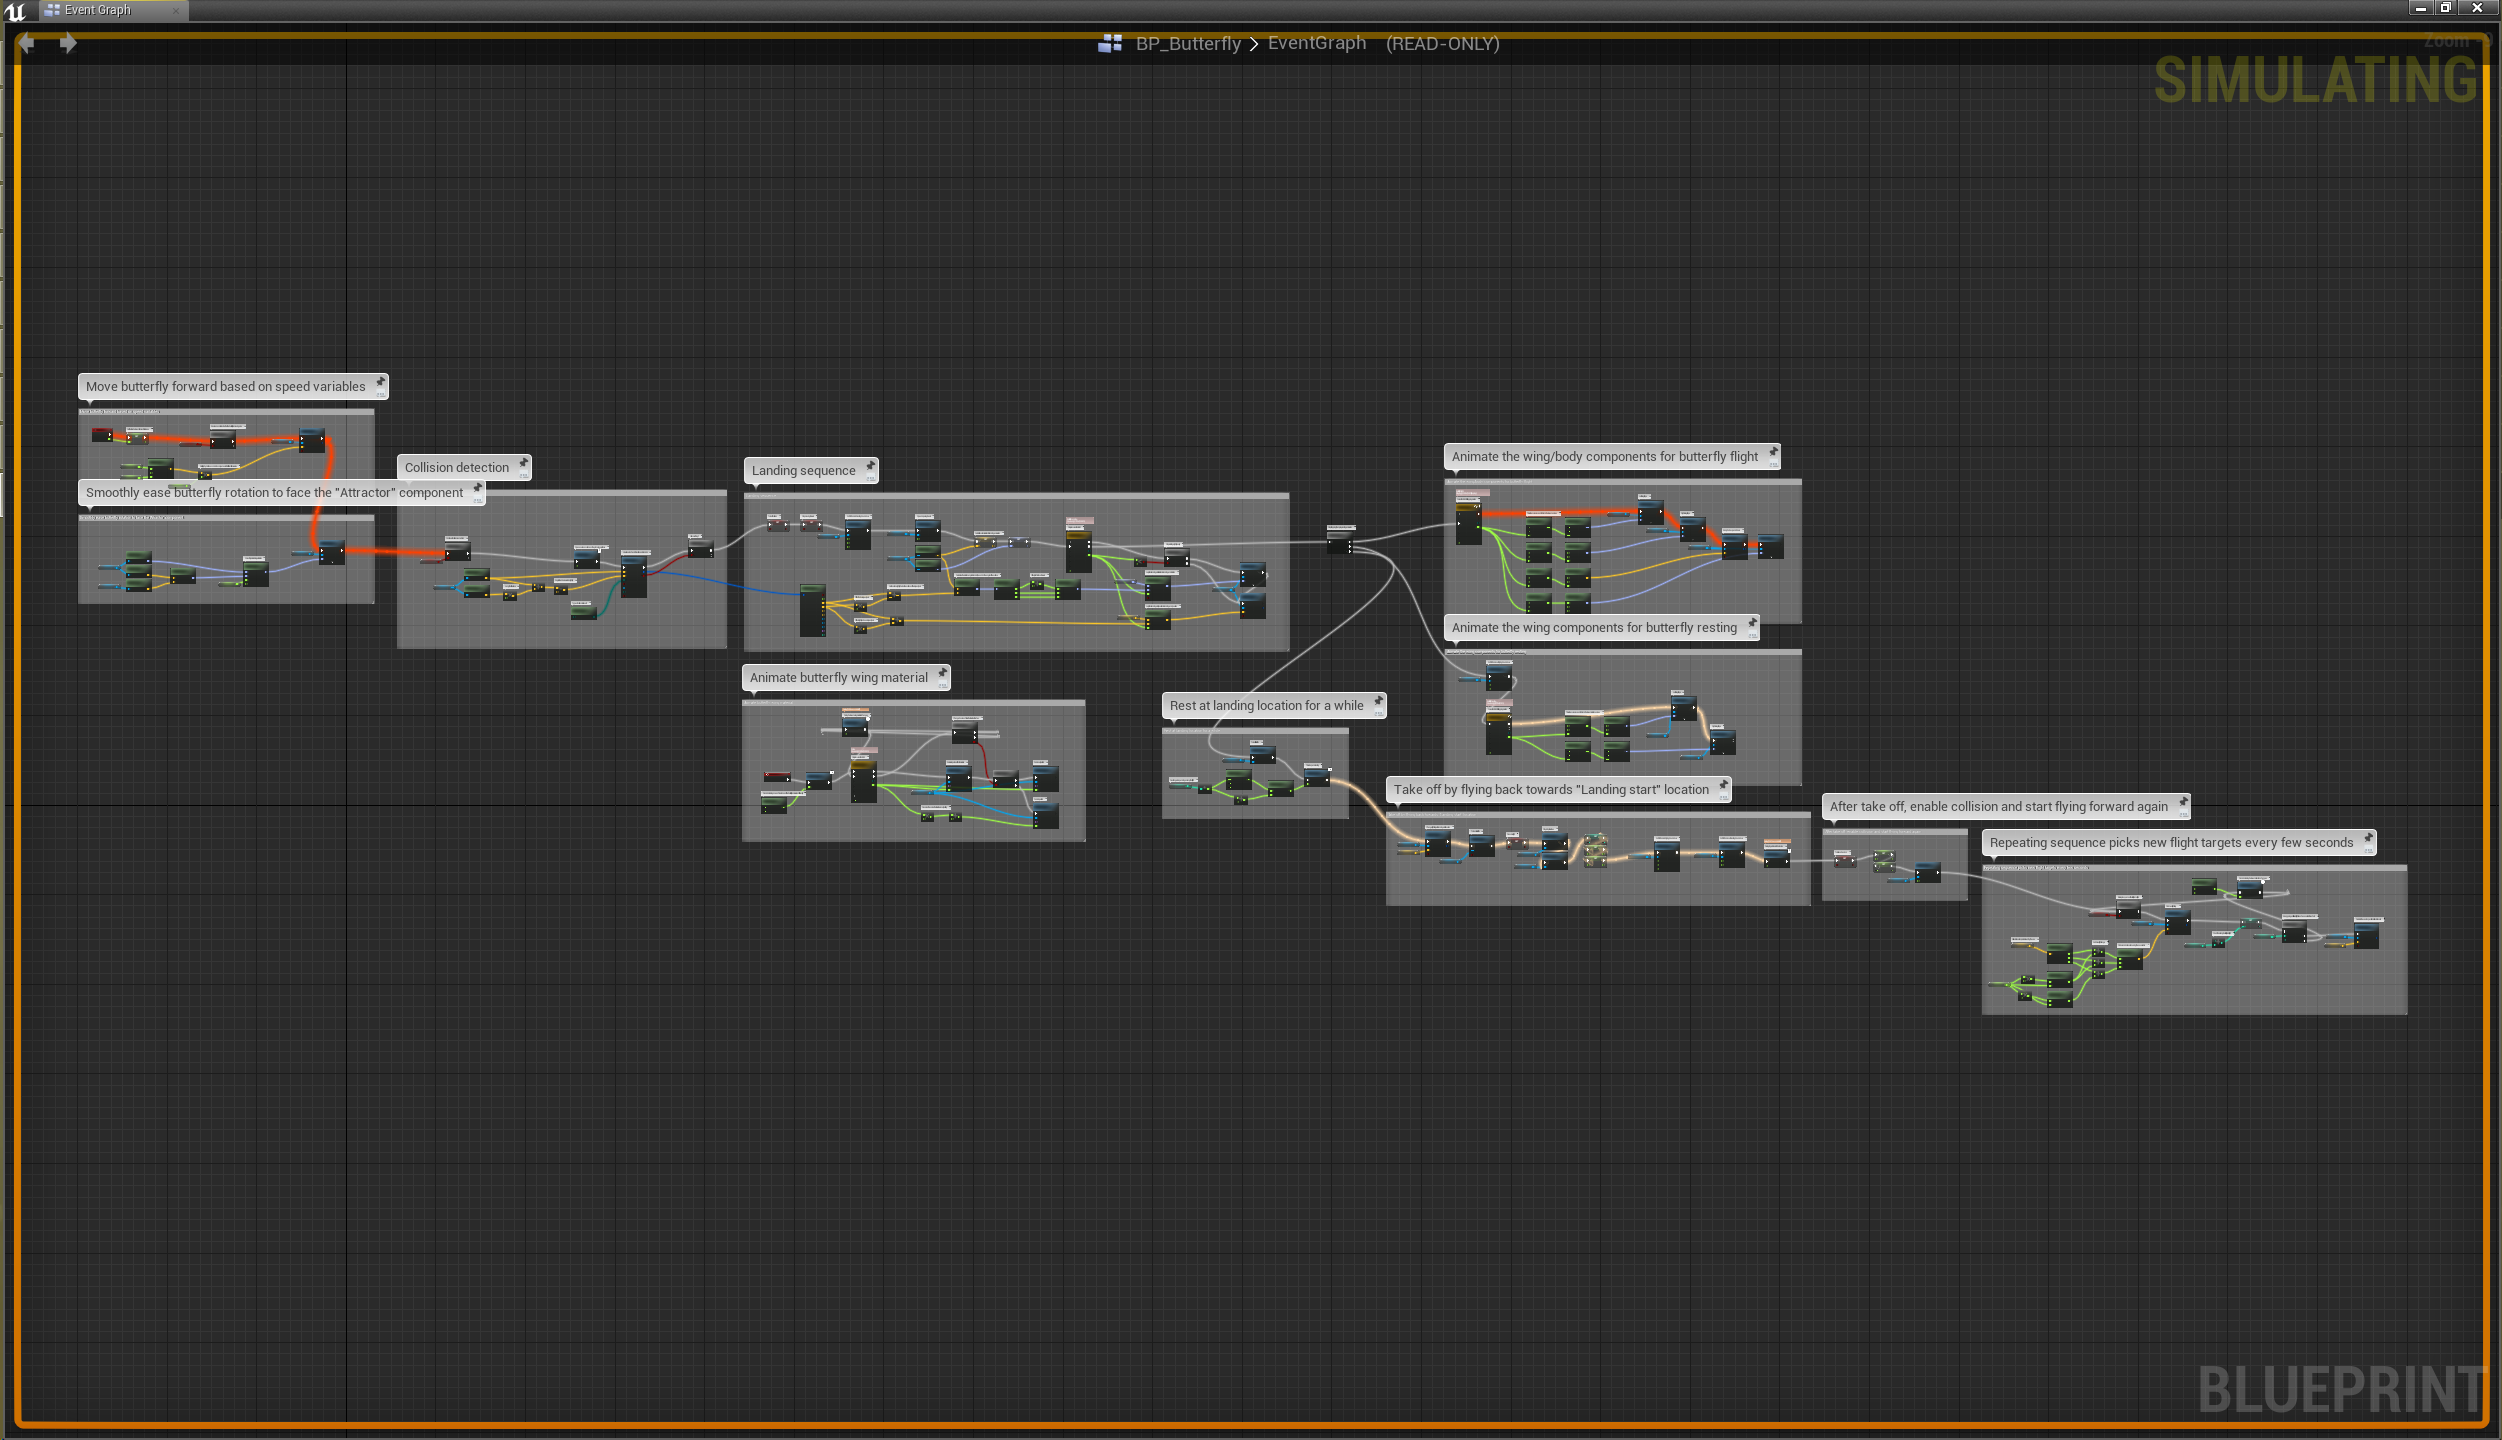
\includegraphics[width=\textwidth]{ue4-blueprint}
\caption{Unreal Engine 4 Blueprint Beispiel}
\end{figure}



\section{Grafik-Engines in Haskell}

\subsection{HGamer3D}

\textit{HGamer3D}\footnote{http://www.hgamer3d.org/} basiert auf (nich kompletten) Haskell-Bindings zu \textit{Ogre}\footnote{http://www.ogre3d.org/}. Ogre ist eine objektorientierte Open-Source Grafik-Engine geschrieben in C++. Ohne weiter auf die Fähigkeiten der Ogre Engine einzugehen, stellt sich oft die Adaptierunung von imperativen Bibliotheken auf funktionale Konzepte als aufwändig und nicht immer optimal heraus. Insbesondere das Erzeugen von Bindings zu komplexen \acsp{API}s ist immer noch eine hohe Hürde.

Auch wenn Ogre als Framework viele Strukturen und Lösungsansätze für gängige Probleme in der 3D Computergrafik und Spieleprogrammierung bereitstellt, ließen sich viele Ansätze auch direkt funktional umsetzen, ohne große und schwerfällige \acsp{API}s zähmen zu müssen.

Zum Beispiel verfolgen beide Welten zum Teil gänzlich andere Grundprinzipien. So sind Daten in Haskell prinzipiell unveränderlich während in C++ Daten prinzipiell veränderlich sind. Haskell erlaubt unter anderem deswegen andere Ansätze der Nebenläufigkeit (Concurrency). Speziell Nebenläufigkeiten stellen immer noch in komplexen Softwareprojekten eine große Hürde dar. Die Adaption einer C++-Biblithek kann das Ausnutzen vieler Vorteile von Haskell behindern (weitere Ausführungen in \fref{sec:warum-haskell}).

Zusätzlich entstehen durch Bindings zu externen Biblitheken neue Abhängigkeiten, die oft eine Anpassung der Tool-Chain erfordern, da sie nicht in das bestehende Ökosystem passen. Dies erhöht die Komplexität des Gesamtsystems. Die Erfahrung des Autos hat gezeigt, dass eigentlich jedes externes Binding früher oder später zu Komplikationen führt, spätestens dann, wenn die Anwendung die Entwicklungsumgebung verlässt. Doch lässt sich nicht jede Abhhängigkeit zu anderen Sprachen vermeiden. Insbesondere in der Grafikprogrammierung mit OpenGL werden die eigentlichen Bindings zu der OpenGL-API benötigt. Zusätzlich muss noch ein platformabhängiger Render-Kontext erzeugt werden.

Meinung des Autors: Es sollten möglichst wenige Fremdabhängigkeiten aus anderen Sprachen genutzt werden, leider ist dies nicht immer möglich (Weitere Ausführungen in \fref{sec:probleme-haskell}). Mit den Ogre Bindings wird die eine komplexe schwer funktional bezwingbare \acs{API} (z.B. OpenGL) mit einer anderen ersetzt.

\subsection{LambdaCube 3D}

\textit{LambdaCube 3D}\footnote{https://lambdacube3d.wordpress.com/} ist eine in Haskell definierte und beeindruckende \ac{DSL}, die es erlaubt Grafikanwendungen bis hin zum Shader komplett in Haskell zu formulieren. Da OpenGL eine komplexe und übersichtliche \acs{API} ist, ist die \ac{DSL} entsprechend komplex und unübersichtlich. Zusätzlich basiert das OpenGL Backend noch auf der Version 3.2. Die Dokumentation beschränkt sich auf den Blog und eine handvoll Beispielen, so dass es schwer ist einen Zugang zu der DSL zu erhalten.

Aber generell stellt sich die bei OpenGL die Frage, wie sinnvoll es ist die komplexe \acs{API} in einer anderen Sprache komplett abzubilden, mit all ihren erlaubten und nicht erlaubten Zuständen, die zusätzlich noch treiberspezifisch sind. Hinzu kommen diverse Erweiterungen, die oft Verhaltensweisen der \acs{API} massiv beeinflussen.

Die persönliche Einschätzung des Autors ist, dass sich OpenGL nicht in einem vertretbaren Aufwand komplett abbilden lässt. Der Aufwand wäre ungefähr mit dem vergleichbar, den Grafikkartenhersteller bei der Implementierung ihrer Grafikkartentreiber betreiben (weitere Ausführungen in \fref{chap:modern-opengl}). Deswegen sollte eine Auswahl der direkten OpenGL Bindings getroffen werden um sie punktuell in funktionale Konzepte zu gießen.

% \subsection{Elm}

% \subsection{Gloss}
% Gloss (2d) ist ein schönes Beispiel dafür wie sich mit einem OpenGL backend und mit der konzentration auf das wesentliche eine klare funktionale api schaffen lässt die einfach anzuwenden ist.

% \cleardoublepage

%%%%%%%%%%%%%%%%%%%%%%%%%%%%%% Überblick Modern OpenGL (4.0+)
\chapter{Überblick über Modern OpenGL}
\label{chap:modern-opengl}

\section{Von Fixed Pipeline zu Shadern}
Mit der Abkehr von der Fixed Pipeline begann die Ära von Modern OpenGL. Seit dem ist es möglich mit eigenen Shader-Programmen, in OpenGL meist geschrieben in GLSL, die einzelnen Stufen der Renderpipline anzupassen. Anfangs beschränkten sich die Stufen auf den Vertex sowie Fragment Shader. Im Laufe der Zeit sind jedoch eine Vielzahl von weiteren programmierbaren Shader-Stufen hinzu gekommen.

\begin{wrapfigure}{r}{0.5\linewidth}
\begin{centering}
	
\includegraphics[width=.5\textwidth]{OpenGL_Nov14}
\end{centering}
\end{wrapfigure}

Die Abkehr von der Fixed Pipeline erlaubte völlig neue Konzepte im Echtzeit-Rendering, anfangen von eigenen, anstatt fest vorgegeben, Beleuchtungsmodellen (siehe \fref{chap:pbr}) hin zu ausschließlich Fragment Shader basierten Grafikdemos\footnote{https://www.shadertoy.com/view/Xtf3Rn} sowie gänzlich neuen Echzeit-Rendering Konzepten\footnote{http://iquilezles.org/www/articles/raymarchingdf/raymarchingdf.htm}.

Während ursprünglich der Szene-Graph fest von OpenGL vorgegeben war und Vertices mindestens einmal jeweils und \textit{einzeln} von der CPU auf die GPU geladen werden mussten, änderte sich auch dies fundamental. Mit dem Ende der Fixed Pipeline wurden auch Buffer-Objekte immer wichtiger, so dass sich ganze Speicherbereiche direkt befüllen oder manipuliert ließen. Der Overhead, Vertices zur Grafikkarte zu schicken, reduzierte sich entsprechend deutlich. Inzwischen gibt es eine Vielzahl von unterschiedlichen Buffer-Typen für unterschiedliche Zwecke, die es sogar erlauben vollständig von Compute Shadern befüllt werden zu können.

Schließlich konnte der bis dato wesentliche Flaschenhals und limitierende Faktor, der Bus zur Grafikkarte, optimal genutzt werden, und war oft nur noch in initialen oder sporadischen Befüllungsvorgängen limitierend. Wie so oft tat sich entsprechend ein neuer Engpass auf. Dieser lag nun, und liegt oft noch immer, in der Implementierung der API, dem Treiber.

\section{Treiber Overhead \& Flexibilität}
\label{sec:overhead-und-flexibilitaet}

Dabei ist die OpenGL API und ihre Treiberimplementierung nicht per se ein Flaschenhals, doch erlaubt die gewachsene und rückwärtskompatibel gehaltene API unterschiedliche Pfade zum annähernd gleichen Ziel. Einige ältere Pfade bringen oft mehr Overhead mit sich, neuere erlauben die effektive Reduzierung der API Aufrufe (siehe \fref{fig:opengl-pfade}). \warn{erhöhung Flexibilität erwähnen} Die \ac{AZDO} Initiative von AMD, nVidia und Intel versucht seit ein bis zwei Jahren die schnelleren Pfade bei den Entwicklern bekannter zu machen. In einem knappen Überblick im folgenden dargestellt und in \fref{chap:haskell-modern-gl} auf ein mögliches Zusammenspiel mit Haskell genauer analysiert.

\begin{figure}
	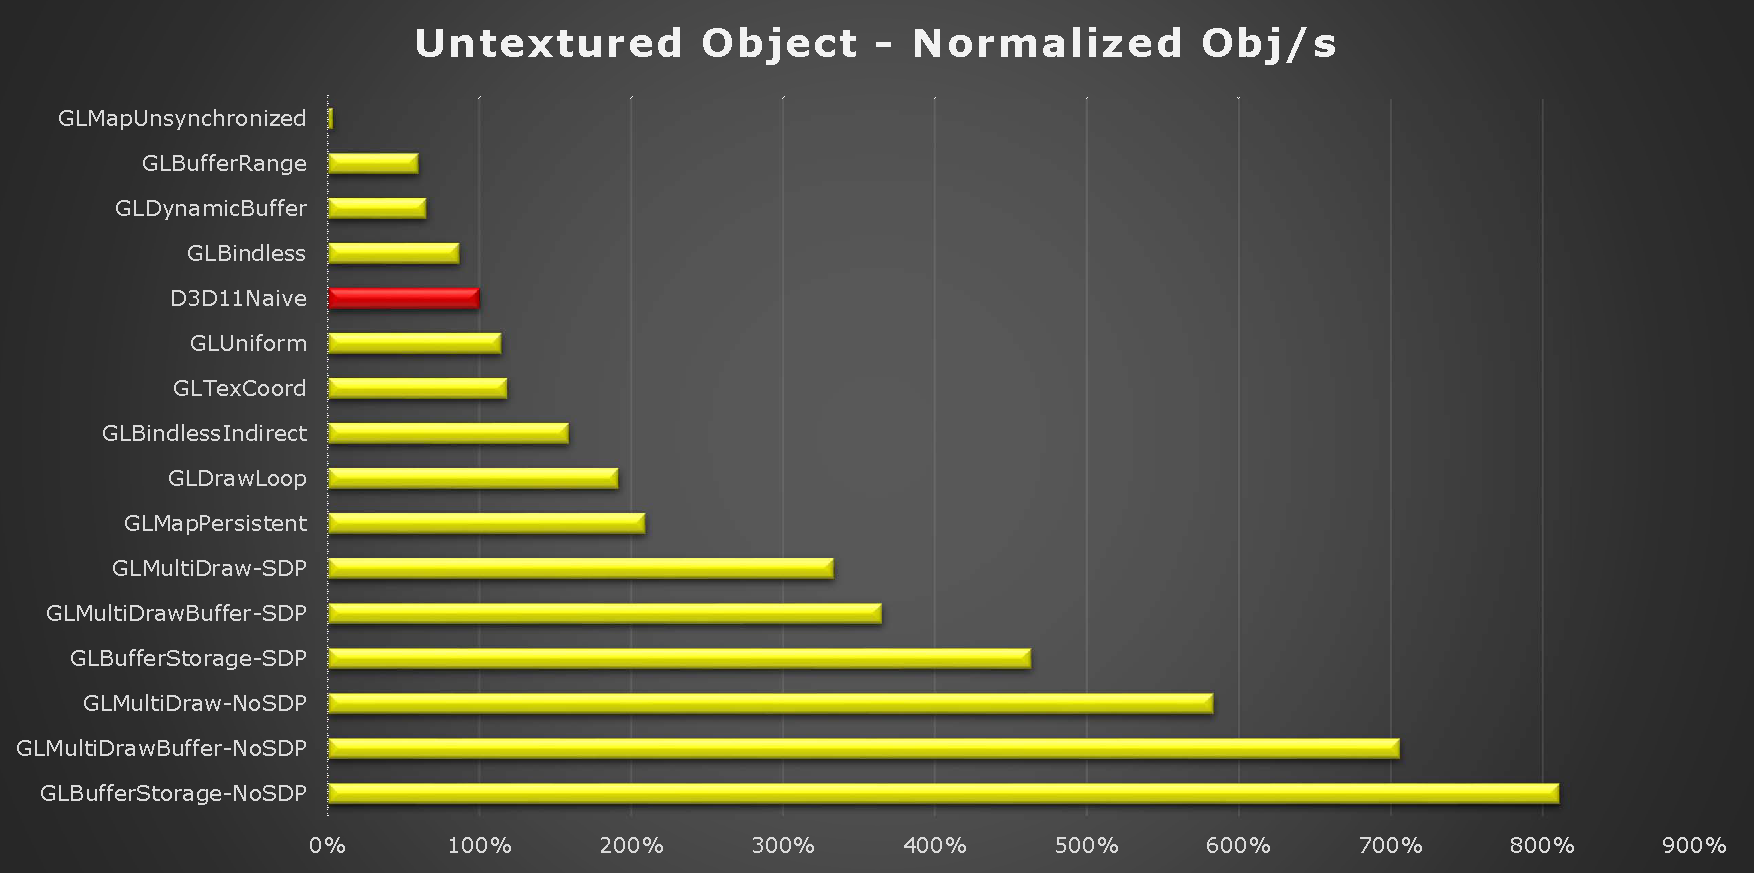
\includegraphics[width=\textwidth]{opengl-spread}
	\caption[Unterschiede in den OpenGL Renderpfaden]{Unterschiede in den OpenGL Renderpfaden \parencite[Seite 98]{Everitt2014}}
	\label{fig:opengl-pfade}
\end{figure}

\paragraph{\acl{MDI}} 
\ac{MDI} beschreibt das Ausführen von mehreren Draw-Calls mit einen API Aufruf. Anstatt für jedes Objekt die notwendigen Aufrufparameter des Draw-Calls separat anzugeben, werden die für alle Objekte notwendigen Parameter in einem OpenGL Buffer (\textit{Command Buffer}) zusammengefasst. Der einzelne indirekte Draw-Call entspricht im wesentlichen nur noch einem Aufruf mit einem Zeiger auf den Inhalt des Command Buffers. Die Parameter können entweder von der CPU aus bestimmt werden oder direkt auf der GPU (z.B. durch View-Frustum Culling auf der GPU). Das Konzept des indirekten Renderns fasst das indexbasierte Rendern und instanziiertes Rendern zusammen\footnote{https://www.opengl.org/wiki/Vertex\_Rendering\#Indirect\_rendering}. Der Command-Buffer in Verbindung mit dem Draw-Call beschreibt ausschließlich die Gestalt des für allen Objekte gemeinsamen \textit{Vertex}-Buffers. Da nun für jedes Objekt kein seperater Draw-Call ausgeführt wird, können auch keine individuellen Daten per Object (zum Beispiel Transformationsmatrizen) an die Shader übergeben werden. Das macht es erforderlich entsprechende Daten gebündelt in einem Array oder \ac{SSBO} dem Shader zu übergeben. Der indizierte Zugriff kann im Shader dann über eingebaute Variablen erfolgen. Dies reduziert zusätzlich den Overhead.

\paragraph{\acl{DSA}} Ein weiterer Schritt zur Reduzierung des Treiber Overheads ist die \ac{DSA} Erweiterung von OpenGL \parencite{Killgard2014} die in den nächsten Jahren mit OpenGL 4.5 Einzug halten wird. Die unterschiedlichen OpenGL Objekte besitzen meistens einen eigenen internen Zustand. Soll dieser Zustand aktualisiert oder abgefragt werden, müssen die Objekte zuvor über Selektoren gebunden werden. Dies ist oft nicht nur fehleranfällig sondern sorgt für wenig intuitiven und lärmenden Quelltext. Zusätzlich erhöht es den API Overhead. 

Mit \ac{DSA} fällt das Selektieren von Objekten vor dem Zugriff auf den Zustand weg und es werden neue Operationen bereit gestellt, die das entsprechende OpenGL Objekt als Parameter erwarten. So lässt sich der Zustand abfragen und manipulieren ohne dass das Objekt vorher im globalen Zustand gebunden werden muss. Dies reduziert den Overhead etwas. Im wesentlichen vereinfacht es die Programmierung mit OpenGL Objekten und erlaubt die Kapselung von Funktionalitäten und erleichtert damit die Umsetzung von komponierbaren Bibliotheken \fref{chap:haskell-modern-gl}.

\paragraph{Separate Program Objects} Auch wenn \ac{DSA} erst mit OpenGL 4.5 breiten Einzug ins \textit{Core} Profil genommen hat, fand die Erweiterung |ARB_separate_program_objects| \parencite{Killgard2011} schon mit Version 4.1 ihren Weg in das \textit{Core} Profil. Zuvor mussten die unterschiedlichen Shader Stufen (Vertex, Geoemetry, Fragment usw.) in ein monolithisches Programm übersetzt werden. Mit der Erweiterung können die einzelnen Stufen unabhängig von einander übersetzt werden. Die Program-Objekte lassen sich dann, unter der Berücksichtungen der Schnittstellen, frei zu einer Programm-Pipeline zusammen setzen. Zusätzlich führt die Erweiterung \ac{DSA} für die Program-Objekte ein, so dass nicht mehr vor der Uniform-Variablenzuwesung die Shader-Objekte gebunden werden müssen. Stattdessen können die Zuweisungen direkt mit dem Program-Objekt durchgeführt werden \warn{link section: \fref{chap:haskell-modern-gl}}.

% ### http://www.g-truc.net/post-0320.html

\section{Vulkan}

\textit{Vulkan} (vormals \textit{glNext}) und \textit{SPIR-V} ist der nächste Schritt (oder Versuch) der \textit{Khronos Group} sich der über Jahrzente gesammelten Altlasten der OpenGL-API zu entledigen. Vulkan wurde im März 2015 als frischer Neustart der Grafik-API angekündigt. Noch ist die Spezifikation am entstehen, aber das erklärte Ziel von Vulkan ist die Reduzierung des CPU Overheads, die breitere Ermöglichung von Multi-Threading und die Abschaffung des impliziten OpenGL Context hin zu einer expliziten API. Neben \textit{Vulkan} wurde \textit{SPIR-V} als eine neue Shader \ac{IL} bzw. Zwischensprache vorgestellt. SPIR-V soll neue Freiräume schaffen eigene Shader-Sprachen sowie Analsyse- und Debuggingtools zu entwickeln\parencite{Olson2015}.

Die Gründe für einen harten Schnitt in der API sind auf zwei Seiten zu suchen. Zum einen ist für den API-Anwender die OpenGL-API wie bereits erwähnt voller Fallstricke. Auf der anderen Seite sind die aktuellen OpenGL Treiber zu einem großen Flickenteppich verkommen. Viele Treiberimplementierungen sind voller Weichen und und Spezialfällen, um bekannte Fehler in der Anwendung der API abzufangen oder potenziell langsame Pfade in schnellere Pfade zu übersetzen \parencite{gamedevnet:glnext}.

\begin{figure*}
\centering
	
\includegraphics[height=2cm]{Vulkan_Mar15}
	
\includegraphics[height=2cm]{SPIR_Nov14}
\end{figure*}



% \cleardoublepage

%%%%%%%%%%%%%%%%%%%%%%%%%%%%%% Funktionale Progammierung & Modern GL
\chapter{Funktionale Programmierung \& OpenGL}
\label{chap:haskell-modern-gl}

Funktionale Programmierung beschreibtich

\ac{DSA} und die verstärkte Verwendung von Buffern für Daten und Kommands (indirectes Rendering) eröffnet neue Spielräume. Währned häufige Foreign Calls in Haskell zu eigenen Bottlenecks führen können (\warn{Beleg}), helfen die Konzepte generell den CPU Overhead zu reduzieren. Während der CPU Overhead im generellen reduziert wird, reduziert sich zusätzlich der Overhead durch die Reduzierung der Foreign Calls. Der gewonnene Spielraum kann für mehr CPU basierte Aufgaben verwendet werden, aber auch um wartungsunfreundliche Kompromisse zwischen Performance und Code-Hygene. Viele Portierungen von Konsole zu PC erwiesen sich oft als zusätzlich aufwändig, da spezielle Optimierungen auf einzelne Anwendungen die Wartung entsprechender Abschnitte deutlich erschwerten (\warn{BELEG}).

- Spielräume
- Kapselung (Uniform StateVars Quine) Koposition (Applikative, Functoren)

% \cleardoublepage

%%%%%%%%%%%%%%%%%%%%%%%%%%%%%% Entwicklung einer Grafikengine in Haskell
\chapter{Überblick über die Engine}
\label{chap:ueberblick-pipeline}

\section{Das Rendersystem}

\warn{Wir beschreiben den sinn und zweck des Renderystems hier. Das Rendersystem ist der Kern der Renderkomponente der Engine. Die Aufgabe des Rendersystems ist eine Eingabe zu einem Bild darzustellen... Im Konkreten Fall erhält das RenderSystem eine Szenenbeschreibung als Eingabe und führt auf Basis dieser alle definierten Schritte um die Szene in der gewünschten Darstellung als Bild zu synthetisieren.}

\subsection{Mealy als Formale Basis}

Das Rendersystem basiert auf dem Konzept eines Mealy Automatens \parencite{Mealy1955}. Ein Mealy Automat ist \ac{FST}, ein spezieller endlicher Automat, der nicht nur seine Eingabesprache vom Eingabeband akzeptiert sondern auch eine Ausgabe auf einem Ausgabeband erzeugt. Ein Transduktor übersetzt die Eingabesprache in eine Ausgabesprache. Bei dem Mealy Automaten als spezielle Form eines \ac{FST} definiert sich die Ausgabe über den momentanen Zustand und die Eingabe auf diesem Zustand. Formal lässt sich ein Mealy Automat $\mathbfcal{M}$ als 6-Tupel wie folgt definieren:

\begin{align}
\mathbfcal{M} = \left( Q, \Sigma, \Omega, \delta, \lambda, q_0 \right)
\label{def:mealy-formal}
\end{align}
\begin{align*}
	\text{mit}\\
	Q &: \text{Endliche Menge von Zuständen} \\
	\Sigma  &:\text{Endliches Eingabealphabet} \\
	\Omega  &:\text{Endliches Ausgabealphabet} \\
	\delta  &:\text{Zustandsübergangsfunktion}\ Q \times \Sigma \rightarrow Q \\
	\lambda &:\text{Ausgabefunktion}\ Q \times \Sigma \rightarrow \Omega \\
	q_0 &: \text{Startzustand}
\end{align*}

Die Definition ließe sich noch um die Menge der finalen Endzustände $F \subseteq Q$ hin zu einem 7-Tupel erweitern. In unserem Konzept verzichten wir auf definierte Endzustände, da wir prinzipiell jede Eingabe akzeptieren. Nicht akzpetierbare Eingaben stellen wir als externe Ausnahmefälle (Exceptions) dar. Ein vereinfachtes Beispiel für eine nicht akzeptierbare Eingabe ist die Eingabe $\bot$, nach der unser gesamtes System in einen undefinierten Zustand $\bot$ wechselt.

\subsubsection{Abstrakte Definition in Haskell}
\label{sec:abstrakte-definition-haskell}

Ein Mealy Automat lässt sich in Haskell abstrakt wie in \fref{lst:haskell-mealy} definieren. {\ttfamily a} beschreibt die Eingabe als Äquivalent zum Eingabealphabet $\Sigma$ der formalen Definition und analog beschreibt |b| die Ausgabe als Äquivalent zum Ausgabealphabet $\Omega$. Die Zustandsübergangsfunktion $\delta$ und die Ausgabefunktion $\lambda$ ergibt sich aus der jeweils konkreten Implementierung des Mealy. Die Menge der Zustände $Q$ wird jeweils von der konkreten Mealy Implementierung gekapselt wie in \fref{lst:state-mealy-beispiel} anhand eines Beispiels veranschaulicht. Aber es lässt sich bereits feststellen, dass die gewählte Form des Mealy Automatens weit mehr als nur ein endlicher Automat ist, da die Mächtigkeit des Ein- und Ausgabealphabets unendlich sein kann, wie dies zum Beispiel bei der Menge der natürlichen Zahlen (abzählbar unendlich) der Fall ist. Daraus folgt zusätzlich, dass auch die Menge der Zustände unendlich sein kann (Zählmaschine).

\begin{haskell}[label={lst:haskell-mealy},caption={[Definition Mealy in Haskell]Definition Mealy in Haskell\protect\footnotemark}]
newtype Mealy a b = Mealy { runMealy :: a -> (b, Maely a b) }
\end{haskell}
\footnotetext{https://hackage.haskell.org/package/machines-0.4.1/docs/Data-Machine-Mealy.html}

Für diese Definition einer Meleay lassen sich einige nützlicher Klassen finden, die wir aber hier überspringen da wir in \fref{sec:konkret-rendersystem} für unsere erweiterte monadische Definition eigene Implementierungen entwickeln werden.

Allgemein lässt sich die Funktionsweise von |Mealy| wie folgt beschreiben: Zu jeder Eingabe |a| erzeugt die Ausfühung von |Mealy| durch |runMealy| eine Ausgabe |b| und einen neuen Mealy-Automaten, der die selbe Eingabesprache in die selbe Ausgabesprache übersetzt. Im einfachsten Fall ist der neu erzeugte Mealy-Automat exakt der gleiche aus dem vorherigen Schritt. Ist dies für das gesamte Eingabealphabet gegeben gilt der Automat als zustandslos.

Für die Konstruktion eines Mealy-Automatens mit lokalem Zustand folgt aus der formalen Definition \ref{def:mealy-formal} die Notwendigkeit einer Zustandsübergangsfunktion $\delta$ und einem Startzustand $q_0$. Hiefür definieren wir uns in \fref{lst:state-mealy-ctr} die Hilfsfunktion |localStateMealy|. Der erste Parameter |s -> a -> (b, s)| beschreibt die Kombination der beiden Funktionen $\delta$ und $\lambda$, der zweite Parameter den Startzustand $q_0$.

\begin{haskell}[label={lst:state-mealy-ctr},caption={[Konstruktion Mealy mit lokalem Zustand]Hilfsfunktion zur Konstruktion eines Mealy-Automatens mit lokalem Zustand}]
localStateMealy :: (s -> a -> (b, s)) -> s -> Mealy a b
localStateMealy stateTransition initState = run initState where
	run state = Mealy (\input -> 
  		let (output, state') = stateTransition state input 
		in (output, stateTransition state'))
\end{haskell}

Mit Hilfe der Funktion |localStateMealy| wird ein Mealy-Automat erzeugt, der bei jeder Ausführung die |stateTransition| Funktion auf die aktuellen Eingabe |input| und den momentanen Zustand |state| anwendet um eine Ausgabe |output| und einen neuen Zustand |state'| zu erzeugen. |output| wird in Verbindung mit dem für die nächste Ausführung neu konstruiertem Meleay-Automaten als Resultat zurück geliefert.

In \fref{lst:state-mealy-beispiel} konstruieren wir einen einfachen Mealy-Automaten der ganzzahlige Eingaben akkumuliert und ausgibt. Abschließend wird in \fref{lst:state-mealy-ausfuehrung} ein Ausführungsbeispiel für |sumMealy| demonstriert.

\begin{haskell}[label={lst:state-mealy-beispiel},caption={[Beispiel Mealy-Automat mit lokalem Zustand]Beispiel Mealy-Automat mit lokalem Zustand}]
sumMealy :: Mealy Int Int
sumMealy = localStateMealy sumInState 0 where
	sumInState state input = (state, state + input)
\end{haskell}

\begin{haskell}[label={lst:state-mealy-ausfuehrung},nolol,caption={Ausführung Mealy-Automat mit lokalem Zustand}]
> let m0 = sumMealy
> let m1 = runMealy m 5
> fst m1
0
> let m2 = runMealy m1 8
> fst m2
5
> let m3 = runMealy m2 0
> fst m3
13
\end{haskell}

\subsection{Konkrete Definition des Rendersystems}
\label{sec:konkret-rendersystem}

\subsubsection{Anforderung}
Ein konkretes Rendersystem soll sich aus mehreren \warn{isolierten} Renderschritten, den Renderpasses, zusammensetzen. Durch die rekursive Definition kann ein Renderpass wiederum ein beliebig komplexes Rendersystem darstellen, so dass zwischen Rendersystem und Renderpass nur semantisch unterschieden wird. Jeder konkrete Pass soll einen konkret definierten Eingabetypen und einen konkret definierten Ausgabetypen besitzen. Ein Renderpass übersetzt die Eingabe in eine Ausgabe und kapselt alle dafür notwendigen Zustände und Vorgänge. Zustandsveränderungen sollen nicht direkt von außen vorgenommen werden können. Zu dem internen Zustand eines Renderpasses können unter anderem benötigte Ressourcen wie Framebuffer oder Shader gehören. Der interne Zustand soll nur vom Renderpass selbst sichbar gemacht werden können, und dass auch nur, wenn (ein Teil-) Zustand vom Renderpass in die Ausgabe geleitet wird. Direkte Veränderungen des internen Zustands sind so von vornherein ausgeschlossen, da in Haskell Daten unveränderlich sind \footnote{ausgenommen über Konstrukte wie MVars oder IORefs}.

Die Definition des Mealy-Typens aus \fref{lst:haskell-mealy} dient als gedankliche Grundlage für die folgende Definition des Rendersystem, da wir mit \ref{lst:state-mealy-ctr} gezeigt haben, wie sich Zustände kapseln lassen. Aus den Anforderungen an das Rendersystem OpenGL-Methoden aufzurufen zu können ergibt sich, dass wir das Konzept des Mealy-Typen noch um einen monadischen Basistypen erweitern müssen, damit wir beispielsweise Operationen in der |IO| Monade ausführen können. Damit wir uns auf keinen konkreten monadischen Typen festlegen müssen, konstruieren wir unser Rendersystem als einen monadischen Transformator (Monad-Transformer). Die Form des monadischen Transformators erlaubt es Operationen aus einer anderen Monade, der Basismonade, in unsere Ausführung zu heben (lift). So können wir unserem Rendersystem zum Beispiel über eine |Writer|-Monade die Fähigkeit verleihen Vorgänge zu protokollieren oder über deine |Reader|-Monade können sich die Renderschritte eine unveränderliche Umgebung (Environment) teilen. Durch das sogenannte Stacken von Monaden ist es möglich die Eigenschaften der unterschiedlichsten Monaden unter einer Monade zusammenzufassen, es entsteht ein Monad-Stack.

\subsubsection{Definition}

Aus den oben gegebenen Anforderungen kann jetzt die Definition für |RenderSystem| in \fref{lst:definition-rendersystem} formuliert werden. |m| entspricht der Basismonade, |i| ist der Typparameter für die Eingabe in das Rendersystem und respektive |o| der Typparameter für die Ausgabe. Das Ausführen eines |RenderSystems| liefert, im Gegensatz zum Mealy-Automaten, als Ergebnis eine monadische Operation mit der Ausgabe |o| und dem neuen |RenderSystem| für die nächste Ausführung. In \fref{lst:rendersystem-beispiel-reader} wird ein einfaches zustandsloses |RenderSystem| auf Basis der |Reader|-Monade definiert und in \fref{lst:rendersystem-ausfuehrung-beispiel} exemplarisch ausgeführt. Das |RenderSystem| gibt den momentanen Integerwert der Umgebung auf stdout aus und liefert den Eingabewert unverändert zurück. Der Integerwert der Reader-Monade könnte zum Beispiel einen globalen Frame-Counter repräsentieren.

\begin{haskell}[label={lst:definition-rendersystem},caption={Definition Rendersystem}]
newtype RenderSystem m i o = RenderSystem { runRenderSystem :: i -> m (o, RenderSystem m i o) }
type RenderPass = RenderSystem -- nur ein semantischer Alias
\end{haskell}

\begin{haskell}[label={lst:rendersystem-beispiel-reader},caption={Beispiel Rendersystem mit ReaderT IO als Basismonade}]
type PrintPass = RenderPass (ReaderT IO Int) a a
printFrame :: PrintPass a a
printFrame = RenderSystem (\i -> do
	env <- ask 
	print (show ask)
	return (i,printFrame))
\end{haskell}

\begin{haskell}[label={lst:rendersystem-ausfuehrung-beispiel},caption={Ausführungsbeispiel Rendersystem}]
> let r0 = runReaderT (runRenderSystem printFrame "Hallo") 0
> fst r0
0
"Hallo"
> let r1 = runReaderT (runRenderSystem r0 "Welt!") 1
> fst r1
1
"Welt"
\end{haskell}

Da wir in der praxis unterschiedliche Formen von |RenderPass|es konstruieren werden, definieren wir uns in \fref{lst:renderpass-ctr} Hilffunktionen für die Konstruktion der drei wesentlichen Ausprägungen: 1. zustandslos und unveränderlich, 2. zustandsbehaftet unveränderlich und 3. voll dynamisch.

\begin{haskell}[label={lst:renderpass-ctr},caption={Konstruktoren für einen RenderPass}]
-- 1. zustandslos und unveraenderlich
mkStaticRenderPass :: Monad m => (i -> m o) -> RenderPass m i o
mkStaticRenderPass f = r where r = RenderSystem (liftM (,r) . f)

-- 2. zustandsbehaftet und unveraenderlich
mkStatefulRenderPass :: Monad m => (s -> i -> m (o,s)) -> s -> RenderPass m i o
mkStatefulRenderPass f = go where
  go s = RenderSystem (\i -> do
    (o, t) <- f s i
    return (o, go t))

-- 3. voll dynamisch
mkDynamicRenderPass :: (i -> m (o, RenderPass m i o)) -> RenderPass m i o
mkDynamicRenderPass = RenderSystem
\end{haskell}


%%%
% Klassen
%%%

\subsubsection{Klassen-Instanzen}
\label{sec:rendersystem-klassen-instanzen}

In \fref{sec:abstrakte-definition-haskell} wurde bereits erwähnt, dass sich für den Mealy-Typen nützliche Klassen-Instanzen implementieren lassen. Die konkreten Implementierungen für den Mealy-Typen wurden übersprungen aber wir werden in diesem Kapitel wesentlichen äquivalente Implementierungen für unseren Typen |RenderSystem| entwickeln. Aus Platzgründen werden nur die jeweils minimal notwendigen Definitionen angegeben, vollständige Definition finden sich im Modul |RenderSystem|. Praktische Anwendungen werden mit unter in \fref{chap:anwendungsbeispiele} gegeben, doch kann auch hier aus Platzgründen keine umfassende Übersicht gegegeben werden. Umfassende Beispiele finden sich ebenso im Projekt beispielsweise im Modul |Yage.Rendering.Pipeline.Deferred|.


%%%
% Functor
%%%

\paragraph{Functor} 
Funktoren, im Folgenden Functor genannt, beschreiben in der Kategorientheorie eine strukturerhaltene Abbildung (Homomorphismus) zwischen zwei Kategorien. In Haskell ist die Klasse der Functoren wie in \fref{lst:class-functor} definiert. Das erste intuitive Verständnis eines |Functor|s in Haskell ist eine Containerstruktur deren Inhalt von einem Typen |a| auf den Typen |b| überführt werden kann, ähnlich dem |map| für die Listen. Zur Klasse der Functoren gehören darüber hinaus noch weit mehr Strukturen. Zum Beispiel lassen sich auch die Ergebnisse von Funktionen homomorph in eine andere Kategorie überführen ohne die Struktur der Berechnung zu verändern.

\begin{haskell}[label={lst:class-functor},caption={Functor Klasse\protect\footnotemark},nolol]
class Functor f where
  fmap :: (a -> b) -> f a -> f b 
\end{haskell}
\footnotetext{http://hackage.haskell.org/package/base-4.7.0.2/docs/Data-Functor.html}

\Fref{lst:rendersystem-functor} definiert eine Functor Instanz für den |RenderSystem| Typen. Beschrieben wird die Überführung des Ergebnistypens |o| in einen neuen Ergebnistypen |c| (siehe konkrete Signatur für |fmap|). Die Implementierung verdeutlich, dass die Struktur der Berechnung nicht verändert wird. Es wird lediglich der Ausgabetyp des |RenderSystem| in einen neuen Ausgabetyp überführt. Diese Functor Instanz ermöglicht es beispielsweise den Ausgabetypen eines |RenderPass|es, mit Hilfe einer Tranformationsfunktion |f| als Adapter, auf den Eingabetypen eines nachfolgenden |RenderPass| zu überführen.

\begin{haskell}[label={lst:rendersystem-functor},caption={Functor Instanz für RenderSystem}]
instance Monad m => Functor (RenderSystem m i) where
  fmap :: (o -> c) -> RenderSystem m i o -> RenderSystem m i c
  fmap f (RenderSystem sys) = RenderSystem (sys >=> \ (o,sys') -> return (f o, fmap f sys'))
\end{haskell}


%%%
% Applicative
%%%

\paragraph{Applicative}
Applikative, im Folgenden Applicatives, sind eine spezielle Ausprägung von Functoren. Ein Applicative wird über zwei Operationen definiert: |pure| bettet einen Wert in den Kontext |f| ein und der Sequenz-Operator |(<*>)| wendet eine Berechnung im Kontext |f| auf einen Wert in |f| an und kombiniert das Resultat \parencite[Kapitel~2]{Paterson2008}. Applicative sind weniger mächtig als Monaden, da sie nur das Sequenzieren von kontextfreien Operationen erlauben. Sie werden gerne dazu verwendet kleine Bausteine als Kombinatoren zu bauen um sie kontextfrei aufeinander anzuwenden. In Haskell sind Applicatives wie in \fref{lst:class-functor} definiert.

\begin{haskell}[label={lst:class-functor},caption={Applicative Klasse\protect\footnotemark},nolol]
class Functor f => Applicative f where
  pure :: a -> f a
  (<*>) :: f (a -> b) -> f a -> f a
\end{haskell}
\footnotetext{http://hackage.haskell.org/package/base-4.7.0.2/docs/Control-Applicative.html}

Für unser |RenderSystem| definieren wir in \fref{lst:rendersystem-applicative} die Applicative Instanz. Auch hier wird anhand der Implementierung von |(<*>)| deutlich, dass die in |sysf| eingebettete Funktion auf den in |sysa| eingebetteten Wert ohne Berücksichtung des Kontext angewendet wird. |pure| entspricht einem RenderSystem, dass ungeachtet der Eingabe konstant den Wert |b| zurück liefert und unter keinen Umständen das Verhalten wechselt. Mit Hilfe der Appliacative Instanz des |RenderSystem|-Typens können wir mehrere Rendersysteme zu einer größeren Struktur kombinieren, sofern die Rendersysteme nicht von einander direkt abhängen. \Fref{lst:rendersystem-applicative-beispiel} zeigt an einem Beispiel, wie über die Applicative Instanz eine Definition eines RenderSystems . Dieses RenderSystem |sceneToTexture| lässt sich dann über die die Applicative Kombinatoren zu einem RenderSystem kombinieren, dass eine Szene in eine Cubemap rendert. Dynamisch erzeugte Cubemaps werden oft als Environment-Maps (Umgebungstexturen) verwendet, um dynamische Spiegelungen der Umgebung auf Objekten darzustellen.

\begin{haskell}[label={lst:rendersystem-applicative},caption={Applicative Instanz für RenderSystem}]
instance Monad m => Applicative (RenderSystem m i) where
  pure b = r where r = RenderSystem (return . const (b,r))
  RenderSystem sysf <*> RenderSystem sysa = RenderSystem (\i -> do
    (f, mf) <- sysf i
    (a, ma) <- sysa i
    return (f a, mf <*> ma))
\end{haskell}

\begin{haskell}[label={lst:rendersystem-applicative-beispiel},caption={Applicative RenderSystem Beispiel}]
data Cube a = CubeTexture{left,right,top,bottom,front,back :: a}

sceneToTexture :: Camera -> RenderPass IO Scene Texture
sceneToTexture = ...

scene :: Scene
scene = ...

-- Cube with cameras along the +/- world axis directions
cubeViews :: Cube Camera
cubeViews = ...

-- Renders a scene into a cube map
sceneToCubeTexture :: RenderPass IO Scene (Cube Texture)
sceneToCubeTexture = Cube
	`fmap` sceneToTexture (left cubeViews)
	<*> sceneToTexture (right  cubeViews)
	<*> sceneToTexture (top    cubeViews)
	<*> sceneToTexture (bottom cubeViews)
	<*> sceneToTexture (front  cubeViews)
	<*> sceneToTexture (back   cubeViews)
\end{haskell}


%%%
% Profunctor
%%%

\paragraph{Profunctor}
Während die vorhergehenden Klassen nur Operationen auf dem letzten Argument des Typens definierten, gehört unser unser |RenderSystem| Typ auch noch weiteren Klassen an, die sich für die letzten beiden Argumente definieren lassen. Ein Functor in zwei Argumenten wird auch Bifunctor genannt. Jedes Argument gehört einer eigenen Functor-Kategorie an, die auch voneinander unterschiedlich sein können aber nicht müssen. Zusammmen bilden die beiden Functor-Kategorien ($C$ und $D$) eine Produktkategorie ($C \times D$) \parencite{MacLane1998}. Ein spezieller Bifunctor ist der Profunctor, dessen erstes Argument contravariant und zweites Argument covariant ist. Ein covarianter Functor entspricht der üblichen Haskell |Functor| Klasse mit einem Morphismus von der Ausgangskategorie hin zur Zielkategorie. Die Contravarianz entspricht dahingehend einem umgekehrten Morphismus, von der Zielkategorie zur Ausgangskategorie. Die Haskell Definition der Klasse |Profunctor| findet sich in \fref{lst:class-profunctor}

\begin{haskell}[label={lst:class-profunctor},caption={Profunctor Klasse\protect\footnotemark},nolol]
class Profunctor p where
  dimap :: (a -> b) -> (c -> d) -> p b c -> p a d
\end{haskell}
\footnotetext{https://hackage.haskell.org/package/profunctors-3.2/docs/Data-Profunctor.html}

Anschaulicher wird die Funktionsweise eines |Profunctor|s wieder bei der Implementierung der |Profunctor| Instanz für unser |RenderSystem|. Das zweite covariante Argument unseres Bifunctors ist unser Parameter |o| für den Ausgabetypen des |RenderSystems| und wird analog zu der Functor Instanz implementiert, mit |g| als Morphismus. Der neue erste Parameter unseres Bifunctors entspricht dem contravarianten Argument. Der umgekehrte Morphismus |f| wird im Gegenzug auf den Eingabewert angewendet, bevor das entsprechende RenderSystem mit der Eingabe ausgeführt wird. Mit der Profunctor Instanz können wir nicht nur elegant den Ausgabetyp unseres Rendersystems konvertieren, sondern auch auch zu einem allgemein definierten Rendersystem neue Varianten erzeugen die auf unterschiedlichen Eingaben arbeiten, solange wir eine Konvertierungsfunktion für die Eingabe definieren können. Die interne Funktionsweise des Rendersystems bleibt trotz etwaiger Konvertierungen von Ein- und Ausgaben die selbe, es werden lediglich die Schnittstellen einem externen Format angepasst.

\begin{haskell}[label={lst:rendersystem-profunctor},caption={Profunctor Instanz für RenderSystem}]
instance Monad m => Profunctor (RenderSystem m) where
  dimap :: (i -> a) -> (b -> o) -> RenderSystem m a b -> RenderSystem m i o
  dimap f g (RenderSystem sys) = RenderSystem (\i -> do
    (o,sys') <- sys (f i)
    return (g o, dimap f g sys'))
\end{haskell}


%%%
% Category
%%%

\paragraph{Category}

Die |Category| beschreibt die Klasse von Strukturen deren Morphismus sich über beide Argumente komponieren lassen. Die grundlegenste |Category| in Haskell ist die der Funktionen und ihre Komponierbarkeit. Unäre Funktionen |(->)| beschreiben einen Morphismus der das Argument der Funktion einem Funktionswert zuordnet. Unäre Funktionen sind in Haskell analog zur mathematischen Funktionskomposition komponierbar. Dies wird dadurch ausgedrückt, dass unäre Funktionen der |Category| Klasse angehören. In \fref{lst:class-category} wird die Definition der Klasse ausgeschrieben. Sie besteht aus dem Identitätsmorphismus |id| und der rechts zu links Komposition |(.)|.

\begin{haskell}[label={lst:class-category},caption={Category Klasse\protect\footnotemark},nolol]
class Category cat where
  id :: cat a a
  (.) :: cat b c -> cat a b -> cat a c
\end{haskell}
\footnotetext{https://hackage.haskell.org/package/base-4.7.0.2/docs/Control-Category.html}

Auch unser Rendersystem beschreibt einen Morphismus von der Eingabe |i| zur Ausgabe |o|. Folglich gehört auch unser |RenderSystem| Typ der Klasse der Kategorien an. In \fref{lst:rendersystem-category} listet die Implementierng der |Category| Klasse für unser |RenderSystem|. Unser Identitätsmorphismus ist ein Rendersystem, dass die Eingabe unverändert ausgibt. Unsere Komposition ist dadurch implementiert, dass wir zuerst die am weitesten rechts stehende Eingabe |a| in unser rechtes |RenderSystem| eingeben und die entsprechende Ausgabe |b| an das linke |RenderSystem| weiter leiten um die finale Ausgabe |c| zu erhalten. Da die jeweiligen Rendersysteme sich dynamisch verändern können, werden die neu erzeugten RenderSysteme ebenso komponiert (|mbc' . mab'|). 

Die erlaubt es uns auf elegenate Weise unterschiedliche Stufen eines RenderSystems hintereinander zu schalten und zu einem größeren Gesamtsystem zu komponieren. \Fref{lst:rendersystem-komposition-beispiel} zeigt an einem Beispiel, wie sich durch die Komposition zweier unabhängig von einander definierten Textur-Filter ein neuer Filter |bloom| erzeugt werden kann.

\begin{haskell}[label={lst:rendersystem-category},caption={Category Instanz für RenderSystem}]
instance Monad m => Category (RenderSystem m) where
  id = RenderSystem (return . (,id))
  RenderSystem mbc . RenderSystem mab = RenderSystem (\a -> do
    (b, mab') <- mab a
    (c, mbc') <- mbc b
    return (c, mbc' . mab'))
\end{haskell}

\begin{haskell}[label={lst:rendersystem-komposition-beispiel},caption={Beispiel einer Komposition von RenderSystem}]
-- Passes colors with Luma above 'threshold'
lumaFilter :: Float -> RenderSystem IO Texture Texture
lumaFilter treshold = ...

-- Filters 'Texture' with a gaussian-kernel of kernelsize x kernelsize
gaussianFilter :: Int -> RenderSystem IO Texture Texture
gaussianFilter kernelsize = ...

bloom :: RenderSystem IO Texture Texture
bloom = gaussFilter 64 . lumaFilter 0.4
\end{haskell}


%%%
% Semigroup
%%%

\paragraph{Semigroup}

Eine \textit{Semigroup} bzw. eine \textit{Halbgruppe} ist eine algebraische Struktur mit einer assoziativen binären Verknüpfung. Sie gilt als Verallgemeinerung eines Monoiden, für die kein neutrales Element benötigt wird und respektive einer \textit{Group} bzw \textit{Gruppe}, für die kein inverses und kein neutrales Element benötigt wird.

\begin{haskell}[label={lst:class-semigroup},caption={Semigroup Klasse\protect\footnotemark},nolol]
class Semigroup a where
  (<>) :: a -> a -> a -- fuer Monoiden 'mappend'
\end{haskell}
\footnotetext{https://hackage.haskell.org/package/semigroups-0.16.2.2/docs/Data-Semigroup.html}

Die Implementierung in \fref{lst:rendersystem-semigroup} verknüpft die beiden |RenderSystem|e, in dem beide auf der gleichen Eingabe sequenziell ausführt werden. Die Resultate werden abschließend mit |(<>)| verknüpft.

\begin{haskell}[label={lst:rendersystem-semigroup},caption={Semigroup Instanz für RenderSystem}]
instance (Applicative m, Semigroup o) => Semigroup (RenderSystem m i o) where
	sysX <> sysY =  RenderSystem (\i -> liftA2 (<>) (runRenderSystem sysX i) (runRenderSystem sysY i))
\end{haskell}

\Fref{lst:rendersystem-semigroup-beispiel} ist ein Beispiel dafür, wie die Resulate aus mehreren Render-Schritten zu einer größeren assoziative Struktur zusammengefügt werden können. In diesem Fall wird mehrfach |downsample| auf auf einer Textur ausgeführt, um anschließend die herunter gerechneten Texturen zu einer Mipmap-Chain zu kombinieren. 

\begin{haskell}[label={lst:rendersystem-semigroup-beispiel},caption={Beispielanwendung Semigroup für RenderSystem}]
import Data.List.NonEmpty
-- | MipmapChain mit einem Basis Element und einer Liste von Mipmap Stufen
-- Instanz von Semigroup
type MipmapChain = NonEmpty

mkBase :: b -> MipmapChain b
mkBase b = b :| []

downsample :: Int -> RenderSystem IO Texture Texture
downsample factor = ...

generateMipmap :: RenderSystem IO Texture (MipmapChain Texture)
generateMipmap = fmap mkBase id 
	<> fmap mkBase (downsample (2^1)) 
	<> fmap mkBase (downsample (2^2)) 
	<> fmap mkBase (downsample (2^3))
\end{haskell}


%%%
% Arrow
%%%

\paragraph{Arrow}

|Arrows| sind eine weitere abstrakte Darstellungsform von Morphismen. Während |Category| die Komponierbarkeit von Morphismen beschreibt, beschreiben Arrows den Morphismus an sich. In Haskell wird ein Arrow über die Operation |arr| und |first| definiert. Zusätzlich gehört zur Arrow Klasse auch die Kompositionsoperation, welche aber schon durch die Spezialisierung von |Category| definiert ist. |arr| stellt den direkten Bezug zu dem grundlegenden Morphismus der unären Funktionen |(->)| und der Arrow Struktur her und hebt einen einfachen Morphismus in den Kontext des |Arrow|s. |first| ist eine Variante, neben dem gespiegelten |second|, der sogenannten Sideline Operation \parencite[Kapitel 1]{Asada2010}. Über |first| kann ein Morphismus |a b c| auf die erste Komponente des Argumentes angewendet werden, während doe zweite Komponente unverändert durchgereicht wird. Erwähnenswert ist abschließend, dass jeder |Arrow| auch als |Profunctor| dargestellt werden kann \parencite[Kapitel 3]{Asada2010}.

\begin{haskell}[label={lst:class-arrow},caption={Arrow Klasse\protect\footnotemark},nolol]
class Category a => Arrow a where
  arr :: (b -> c) -> a b c
  first :: a b c -> a (b, d) (c, d)
\end{haskell}
\footnotetext{https://hackage.haskell.org/package/base-4.7.0.2/docs/Control-Arrow.html}


\begin{haskell}[label={lst:rendersystem-arrow},caption={Arrow Instanz für RenderSystem}]
instance Monad m => Arrow (RenderSystem m) where
  arr f = RenderSystem (\i -> return (f i, arr f))
  first sys = RenderSystem (\ (b,d) -> do
    (c, sys') <- runRenderSystem sys b
    return ((c,d), first sys'))
\end{haskell}

%%%
% ArrowChoice
%%%

\paragraph{ArrowChoice}

Bevor wir zu einem abschließenden Beispiel für die Anwendung der |Arrow| Implementierung unter Verwendung der Arrow-Notation \footnotemark kommen, werden wir im folgenden noch für unser |RenderSystem| die |ArrowChoice| Klasse implementieren um weitere Möglichkeiten der Arrow Notation nutzen zu können. |Arrow|s die auch |ArrowChoice| implementieren können in der Arrow Notation |if| und |case| Konstrukte als syntaktischen Zucker verwenden. Die Definition der |ArrowChoice| Klasse ist in \fref{lst:class-arrowchoice} angeben. |left| beschreibt dabei eine Operation die eine Operation auf das Argument anwendet, wenn das Argument mit |Left| markiert wurde. Wurde das Argument mit |Right| markiert bleibt es unverändert.

\footnotetext{https://downloads.haskell.org/~ghc/7.8.2/docs/html/users\_guide/arrow-notation.html}

\begin{haskell}[label={lst:class-arrowchoice},caption={ArrowChoice Klasse\protect\footnotemark},nolol]
class Arrow a => ArrowChoice a where
  left :: a b c -> a (Either b d) (Either c d)
\end{haskell}
\footnotetext{https://hackage.haskell.org/package/base-4.7.0.2/docs/Control-Arrow.html\#g:5}

Die Implementierung von |ArrowChoice| für unser |RenderSystem| in \fref{lst:rendersystem-arrowchoice} ist trivial. Wurde die Eingabe mit |Left| markiert, wenden wir unser |RenderSystem| auf die Eingabe an und markieren die Ausgabe wiederum mit |Left|. Mit |Right| markierte Eingaben passieren das RenderSystem unverändert und ohne Seiteneffekte.

\begin{haskell}[label={lst:rendersystem-arrowchoice},caption={ArrowChoice Instanz für RenderSystem}]
instance Monad m => ArrowChoice (RenderSystem m) where
  left sys = RenderSystem (\case
    Left i  -> do
      (b, sys') <- runRenderSystem sys i
      return (Left b, left sys'))
    Right i -> return (Right i, left sys)
\end{haskell}

% \cleardoublepage

%%%%%%%%%%%%%%%%%%%%%%%%%%%%%% Entwicklung einer Grafikengine in Haskell
\chapter{Physically Based Rendering}
\label{chap:pbr}

\acl{PBR} beschreibt ein relativ neues Oberflächenmaterial- und Beleuchtungskonzept in der Spieleindustrie. Es basiert auf dem von Disney vorgestelltem Beleuchtungsmodell \parencite{Burley2012}. Während Disney ein festes Beleuchtungsmodell entwickelte, gibt \ac{PBR} kein festes Regelwerk vor und ist daher vielmehr als ein Paradigma zu verstehen, das erlaubt die Wechselwirkung von Licht, Oberflächen und Betrachter allgemeingültig und akkurat zu simulieren \parencite[Kapitel 1]{Rousiers2014}. Es führt dabei auch kein weiteres Beleuchtungsmodell ein, sondern lässt sich mit unterschiedlichen Approximationen der BRDF nutzen. Nicht desto trotz bedeutet die Umstellung auf ein \ac{PBR} Verfahren eine komplette Umstellung der Produktions- und Renderpipeline. In diesem Kapitel geben wir einen kurzen Überblick über die Prinzipien von \ac{PBR} und Beweggründe, warum es sich lohnen könnte, dieses Konzept praktisch umzusetzen.

\section{Gründe für \ac{PBR}}
\label{sec:pbr-warum}
bla

\section{Grundlagen}
bla

\section{Umsetzung}
bla

\section{Wo wird es eingesetzt?}
Inzwischen wird das Verfahren in allen großen Spieleengines eingesetzt: CryEngine \parencite{Schulz2014}, Unreal Engine 4 \parencite{Martin2012}, Frostbite \parencite{Lagarde2014} und der Engine hinter den Call of Duty Titeln \parencite{Lazarov2011}.

% \cleardoublepage

%%%%%%%%%%%%%%%%%%%%%%%%%%%%%% Anwendungsbeispiele
\chapter{Anwendungsbeispiele}
\label{chap:anwendung}

Es folgt eine exemplarische Implementierung eines Tone-Map Render"-schritts. Die Aufgabe des Render"-schritts besteht darin eine HDR-Textur auf einen vom Monitor darstellbaren RGB Farbraum abzubilden. Die eigentliche Abbildung der Farbwerte wird im Shader |"res/glsl/sampling/tonemap.frag"| vorgenommen und ist hier, mit einem Verweis auf die Implementierung, nicht weiter aufgeführt. Die folgende Implementierung wird schrittweise erläutert und in Teilen aus didaktischen Gründen etwas gegenüber der eigentlichen Implementierung vereinfacht. Der zusammenhängende Quellcode dieses Beispiels findet sich in \fref{lst:tonemap-pass-vollstaendig}.

\paragraph{Ressourcenverwaltung} In der Implementierung wird eine eigene |Resource| Monade zur Verwaltung der Ressourcen auf Basis des |resourcet|\footnote{https://hackage.haskell.org/package/resourcet} Pakets verwendet. In dieser |Resource| Monade lassen sich Ressourcen akquirieren (zum Beispiel mit |glResource|) und über die |Applicative| und |Functor| Instanzen kombinieren. Verlässt das Programm den Kontext der |Resource| Monade, zum Beispiel beim Beenden der Renderloop, werden alle Ressourcen über die registrierte Operation freigegeben.

\paragraph{StateVars} StateVars sind eine einfache Kapselung von zwei IO Operationen, von der eine Operation einen Wert abfragt und und die andere Operation einen Wert setzt. Oft werden StateVars in Verbindung mit externen (foreign) Biblitheken verwendet um veränderliche Zustände zu kapseln. StateVars können als normale Haskell Datenobjekte verwendet werden. Eine Ad-Hoc Implementierung findet sich in \fref{lst:statevar}.

\begin{haskell}[label={lst:tonemap-pass-sig},caption={\texttt{ToneMapPass} Signatur},nolol]
type ToneMapInput = (HDRSensor, Texture2D PixelHDR, Maybe (Texture2D PixelHDR))
type ToneMapOutput = (Texture2D PixelRGB8)
type ToneMapPass = RenderPass ResIO ToneMapInput ToneMapOutput
\end{haskell}

Die Eingabe in unser |RenderPass| ist ein Triple aus |HDRSensor|, einer HDR Textur |Texture2D PixelHDR| und einer weiteren optionalen HDR Textur, die additiv mit der ersten gemischt wird. |HDRSensor| ist Teil einer |HDRCamera| und beinhaltet für das Tone-Mapping benötigte Größen, wie den Weiß-Punkt oder die Belichtung (Exposure). Die Ausgabe ist eine übliche RGB Textur.

\begin{haskell}[label={lst:tonemap-pass-res},caption={\texttt{ToneMapPass} Resourcen Allokation},nolol]
toneMap :: Resource ToneMapPass
toneMap = do
  emptyvao <- glResource
  boundVertexArray $= emptyvao
  fbo <- glResource
  
  pipeline <- [ $(embedShaderFile "res/glsl/sampling/drawRectangle.vert")
              , $(embedShaderFile "res/glsl/sampling/tonemap.frag")]
              `compileShaderPipeline` includePaths
  Just (FragmentShader{..}) <- traverse fragmentUniforms =<< get (fragmentShader $ pipeline^.pipelineProgram)

  outTexture <- liftIO . newIORef =<< createTexture2D GL_TEXTURE_2D (Tex2D 1 1) 1

  return $ mkStaticRenderPass $ \(sensor, sceneTex, mBloomTex) -> do
\end{haskell}

In \fref{lst:tonemap-pass-res}, dem Ressourcenblock des Renderschritts, werden die Ressourcen akquiriert, die zur Ausführung der ab \fref{lst:tonemap-pass-run-resize} beschrieben Routine notwenig sind. Dazu gehören ein Vertex Array Objekt, Framebuffer Objekt und die aus dem Vertex-Shader |drawRectangle.vert| und dem Fragment-Shader |tonemap.frag| erzeugte OpenGL Pipeline\footnote{https://www.opengl.org/wiki/GLSL\_Object\#Program\_pipeline\_objects}. Die Uniform Variablen des Fragment-Shaders werden von |fragmentUniforms| als |StateVar|s gekapselt (siehe Verwendung \fref{lst:tonemap-pass-run-pipeline}). Zusätzlich erzeugen wir uns eine interne |IORef| für die Ausgabetextur. Da die verwendeten OpenGL Texturen\footnote{erzeugt mit \texttt{glTexStorage*}} in ihrer Größe unveränderlich sind, muss für neue Ausgabegrößen entsprechend auch jeweils eine neue Textur erzeugt werden (siehe \fref{lst:tonemap-pass-run-reize}). Dieses Texturobjekt speichern wir uns für den nächsten Aufruf in der |IORef|.

\begin{haskell}[label={lst:tonemap-pass-run-resize},caption={[ToneMapPass Größenanpassung des Framebuffers]\texttt{ToneMapPass} Größenanpassung des Framebuffers},nolol]
    target <- get outTexture
    when (target^.textureDimension /= sceneTex^.textureDimension) $ do
      let V2 w h = sceneTex^.asRectangle.extend
      newtarget <- (\t -> resizeTexture2D t w h) =<< get outTexture
      outTexture $= newtarget
      void $ attachFramebuffer fbo [mkAttachment newtarget] Nothing Nothing
    boundFramebuffer RWFramebuffer $= fbo
\end{haskell}

Gegebenenfalls wird die Ausgabetextur in ihrer Größe an die Größe der Basistextur angepasst. Da die Größenanpassung der Textur intern durch das Erzeugen einer neuen Textur durchgeführt wird, muss die neue Textur noch dem Framebuffer neu angefügt werden (\fref{lst:tonemap-pass-run-resize}).

\begin{haskell}[label={lst:tonemap-pass-run-pipeline},caption={\texttt{ToneMapPass} Zuweisung an Uniform Variablen},nolol]
    boundProgramPipeline $= pipeline^.pipelineProgram

    iScene $= sceneTex
    iBloom $= mBloomTex
    iHdrSensor $= sensor
\end{haskell}

In \fref{lst:tonemap-pass-run-pipeline} wird die erzeugte Shaderpipline für diesen Renderschritt aktiviert und den in |StateVar|s gekapselten Uniform Variablen des Fragment-Shaders Werte zugewiesen.

\begin{haskell}[label={lst:tonemap-pass-run-draw-and-out},caption={\texttt{ToneMapPass} Draw-Call und Textur ausgeben},nolol]
    glDrawArrays GL_TRIANGLES 0 3

    get outTexture
\end{haskell}

Abschließend wird der Draw-Call abgesetzt und die nun von OpenGL gefüllte Textur als Ausgabe zurück gegeben (\fref{lst:tonemap-pass-run-draw-and-out}).

% \cleardoublepage

%%%%%%%%%%%%%%%%%%%%%%%%%%%%%% Analyse
\chapter{Analyse}
\label{chap:analyse}
Argument performance. auch wenn engines und echtzeit performance kritisch sind, gibt es hotspots.
Der Gründer von Epic Games (Unreal Engine) würde 10\% der Performance für 10\% mehr Produktivität opfern \parencite[Seite 20]{Sweeney2006} % Next Mainstream Programming Language


% \cleardoublepage

%%%%%%%%%%%%%%%%%%%%%%%%%%%%%% Ausblick
\chapter{Ausblick}
\label{chap:ausblick}

Im Abschluss dieser Arbeit werden noch kurz offene Felder und weitere Ideen für die Zukunft diskutiert.

\paragraph{Material Graph} Auf Basis des entwickelten Rendering-Frameworks könnte in Zukunft eine Bibliothek zur semi-prozeduralen Erzeugung von Materialien entwickelt werden. Die könnte aus Bausteinen bestehen, die sich mittels eines gerichteten Graphens in Abhängigkeit zueinenader setzten lassen. Eine anschließende toplogische Sortierung der Knoten dient zur Auflösung der Abhängigkeiten. Die Bausteine könnten entweder Texturen als Basis in den Graphen importieren oder prozedural erzeugen. Weitere Bausteine filtern, kombinieren oder manipulieren auf sonstigem Wege ihre Eingangskanäle. Die Form der Definition des Rendersystems aus dieser Arbeit weißt schon eine Struktur auf, die das ermöglichen würde. Die Idee stammt aus diversen Material Editoren, wie dem des \textit{Unreal 4 Editors} (siehe \fref{fig:material-graph}) oder \textit{Shader Forge}\footnote{http://www.acegikmo.com/shaderforge/} oder \textit{Substance Designer}\footnote{https://www.allegorithmic.com/products/substance-designer}.

\begin{wrapfigure}{r}{0.5\linewidth}
\centering
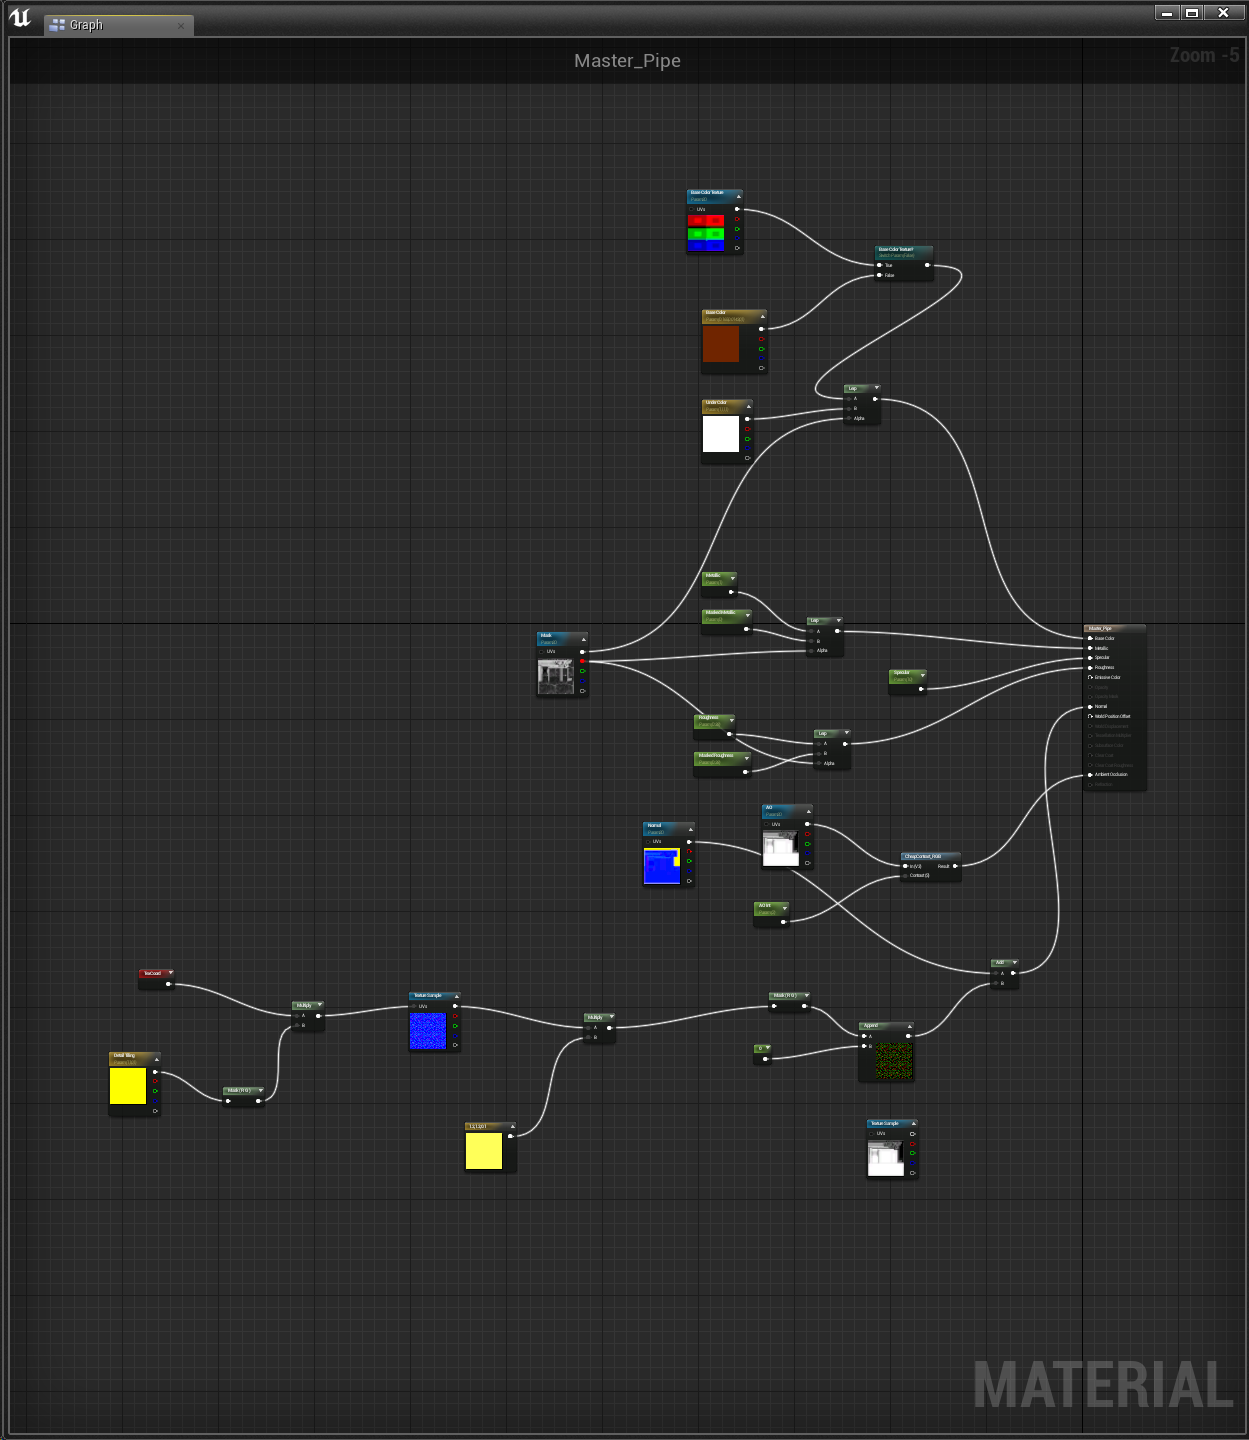
\includegraphics[width=0.5\textwidth]{ue4-material-graph}
\caption{Unreal Engine 4 \mbox{Material Graph}}\label{fig:material-graph}
\end{wrapfigure}

\paragraph{GUI-Framework}\label{sec:gui-framework} Haskell mangelt es an in ausschließlich in Haskell definierten und platformunabhängigen \acsp{GUI}. Bestehende Bindings zu \acs{GUI}-Frameworks sind oft nur unter großem Aufwand, zum Beipsiel unter Windows oder OS X, für einzurichten. Hinzu kommt, dass diese externen Frameworks imperativ gefärbt sind und deswegen oft noch funktional adaptiert werden müssen. Ein ausschließlich auf funktionalen Konzepten (z.B. \ac{FRP}\footnote{http://stud.fh-wedel.de/\~inf9912/research/20131207-info-seminar-frp-netwire/}) basierendes \acs{GUI}-Framework ohne Abhängigkeiten die sich als Hürde für Entwickler und Anwender herausstellen, brächte einige Vorteile für Akzeptanz von Haskell mit sich. Lässt sich erst einmal auf breiter Front produktive Anwendungssoftware entwickeln, die auch nicht nur hinter verschlossenen Türen verwendet wird, dürfte das weitere Aufmerksamkeit von Entwicklern auf Haskell ziehen. Oft wird von außenstehenden Entwicklern berechtigterweise angebracht, dass es wenige "`Real World"' Anwendungen von Haskell gibt oder wenn es sie gibt, sie nur versteckt hinter verschlossenen Türen existieren und nicht bewusst wahrgenommen werden, wie dies zum Beispiel bei Server-Anwendungen der Fall ist.

\paragraph{Vulkan \& SPIR-V} Zu den Kernzielen von \textit{Vulkan} gehören zum einen die Reduzierung des \acs{API}-Overheads und die Reduzierung der \ac{API} auf die modernen und wesentlichen Funktionen (\fref{sec:vulkan}) aber auch zum anderen in der Entwicklung einer expliziten \acs{API}. Sollte dies gelingen, drüfte sich der Umfang der \acs{API} deutlich reduzieren, und so könnten sich neue Möglichkeiten für die funktionale Adaptierung der Grafik-\acs{API} entwickeln. Die explizite \ac{API} könnte es zum ersten mal bei vertretbaren Aufwand ermöglichen die \ac{API} in einer relativ kompakten \ac{DSL} abzubilden. Da sich Haskell selbst sehr gut zur Definition, Parsen und Übersetzen von Sprachen eignet, könnte mit der Zwischensprache \textit{SPIR-V} sich die Möglichkeit auftun, eine (Teil-) Menge von Haskell direkt nach \textit{SPIR-V} hin zu übersetzen. Beispielsweise mittels der \acf{GHC}-\acs{API}, wie dies bei \textit{GHCJS}\footnote{https://github.com/ghcjs/ghcjs} bereits realisiert it.

% \cleardoublepage

%%%%%%%%%%%%%%%%%%%%%%%%%%%%%% Appendix

\appendix

%%%%%%%%%%%%%%%%%%%%%%%%%%%%%% Bib

%%%%%%%%%%%%%%%%%%%%%%%%%%%%%% Bib
\nocite{*}
\printbibliography[heading=head]



%%%%%%%%%%%%%%%%%%%%%%%%%%%%%% Quellen
\chapter{Quellen}

\section[ToneMapPass]{\texttt{ToneMapPass}}
\label{sec:src-tonemappass}

\begin{haskell}[label={lst:tonemap-pass-vollstaendig},caption={\texttt{ToneMapPass} vollständig}]
type ToneMapInput = (HDRSensor, Texture2D PixelHDR, Maybe (Texture2D PixelHDR))
type ToneMapOutput = (Texture2D PixelRGB8)
type ToneMapPass = RenderPass ResIO ToneMapInput ToneMapOutput

toneMap :: Resource ToneMapPass
toneMap = do
  emptyvao <- glResource
  boundVertexArray $= emptyvao

  pipeline <- [ $(embedShaderFile "res/glsl/sampling/drawRectangle.vert")
              , $(embedShaderFile "res/glsl/sampling/tonemap.frag")]
              `compileShaderPipeline` includePaths

  Just (FragmentShader{..}) <- traverse fragmentUniforms =<< get (fragmentShader $ pipeline^.pipelineProgram)

  outTexture <- liftIO . newIORef =<< createTexture2D GL_TEXTURE_2D (Tex2D 1 1) 1
  fbo <- glResource
  return $ mkStaticRenderPass $ \(sensor, sceneTex, mBloomTex) -> do
    target <- get outTexture
    when (target^.textureDimension /= sceneTex^.textureDimension) $ do
      let V2 w h = sceneTex^.asRectangle.extend
      newtarget <- (\t -> resizeTexture2D t w h) =<< get outTexture
      outTexture $= newtarget
      void $ attachFramebuffer fbo [mkAttachment newtarget] Nothing Nothing

    boundFramebuffer RWFramebuffer $= fbo

    glDisable GL_DEPTH_TEST
    glDepthMask GL_FALSE
    glDepthFunc GL_ALWAYS
    glDisable GL_BLEND
    glDisable GL_CULL_FACE
    glFrontFace GL_CCW

    boundVertexArray $= emptyvao
    boundProgramPipeline $= pipeline^.pipelineProgram

    iScene $= sceneTex
    iBloom $= mBloomTex
    iHdrSensor $= sensor
    
    glDrawArrays GL_TRIANGLES 0 3

    get outTexture
\end{haskell}

\section[StateVar]{\texttt{StateVar}}
\label{sec:src-statevar}

\begin{haskell}[label={lst:statevar},caption={Definition \texttt{StateVar}}]
data StateVar a = StateVar (IO a) (a -> IO ())

($=) :: StateVar a -> a -> IO ()
(StateVar _ setter) $= a = setter a

get :: StateVar a -> IO a
get (StateVar getter _) = getter
\end{haskell}

\begin{landscape}
\section{Deferred PBR Pipeline Übersicht}
\label{sec:src-pipeline}
\lstinputlisting[language=Haskell]{src/deferred-pbr-pipeline.hs}
\end{landscape}

\chapter[DVD mit Projektquellen]{DVD mit Projektquellen}\label{chap:dvd}

Quellen auf Github mit Entwicklungsumgebung, Windows Binaries und konsolidierten Quellen:
https://github.com/MaxDaten/yage-meta/releases/tag/0.6.1


\chapter{Eidesstattliche Erklärung}
Ich erkläre hiermit an Eides Statt, dass ich die vorliegende Arbeit selbstständig 
und ohne Benutzung anderer als der angegebenen Hilfsmittel angefertigt 
habe; die aus fremden Quellen direkt oder indirekt übernommenen Gedanken 
sind als solche kenntlich gemacht. 
Die Arbeit wurde bisher in gleicher oder ähnlicher Form keiner anderen Prüfungskommission vorgelegt
und auch nicht veröffentlicht.

\begin{flushright}
Ort, Datum  \ Unterschrift (Vor- und Nachnahme)
\end{flushright}


\thispagestyle{empty}
% \cleardoublepage
\null\newpage



\end{document}
